\chapter{Modelo matemático}
\label{cap:descripcionTrabajo}

En este capítulo exponemos un modelo matemático sencillo que da una posible explicación al mecanismo de reproducción y muerte de las células T. Para este algoritmo, hemos supuesto una cantidad mínima de procesos bioquímicos conocidos y, a partir de ellos, hemos logrado un modelo que, a pesar de su simplicidad, es capaz de ajustarse a hechos observados. 

Al final del capítulo se recogen una serie de simulaciones del modelo, así como un análisis de las mismas. 

\section{Introducción}

Como ya sabemos, las células T juegan un papel fundamental en cuanto a la defensa de patógenos se refiere. Una vez que se detecta el patógeno, estas se activan y reproducen de manera rápida para intentar paliar los efectos dañinos producidos por estos agentes. Este proceso de división masiva, la población puede llegar a incrementarse hasta $10^6$ veces, se conoce como \textit{expansión clonal}. Una vez que el patógeno ha sido vencido, los niveles de población se restauran mediante un proceso denominado \textit{contracción clonal}. Aunque durante esta última etapa muchas células T mueren, alrededor de un 5-10\% quedan como células T con memoria, células listas para dar una respuesta más rápida si el mismo patógeno vuelve a aparecer. 

Hechos experimentales demuestran que la aparición de un patógeno no es suficiente para la toma de decisión entre división o muerte de la célula. Las células T continúan dividiéndose en la ausencia de este estímulo o cometen apóptosis cuando este persiste. 
Siguiendo estos hechos, asumiremos en nuestro modelo que estas decisiones vienen determinadas por la competición de dos moléculas inhibidoras: Retinoblastoma (Rb), que previene la expresión de genes necesarios para que la célula pueda continuar el ciclo celular y dividirse, y célula B linfoma-2 (Bcl-2), que bloqueará la muerte celular. También tendremos en cuenta que la las células T se comunican con el exterior gracias a sus TCR y, por tanto, sus decisiones se ven influenciadas por la cantidad de receptores que tengan. Cuantos más receptores, más estímulos serán capaces de percibir.


\section{Hipótesis biológicas y modelo matemático}

En esta sección explicaremos cuáles son las hipótesis de partida y describiremos con detalle las ecuaciones de nuestro modelo. 

\subsection{Hipótesis biológicas} 
\label{subsec:hip_bio}

\subsubsection{La competición entre dos moléculas inhibidoras determina la decisión y la duración de la vida de una célula T}
\label{susubsec:hip_1}
	 
La división celular, así como, el programa de apóptosis están bloqueados al comienzo de la formación de las células T. Por una parte, Rb frena el inicio del ciclo celular. Para desactivar esta función y que la célula pueda dividirse, es necesario que un número suficiente de estas moléculas sea fosforilado \footnote{Fosforilación: adición de un grupo fosfato a cualquier otra molécula.}.  Por otra parte, las proteínas Bcl-2 bloquean el camino hacia la muerte celular durante infecciones agudas, mediante la contención de la acción de otras proteínas como \textit{Bax} o \textit{Bim}.


\begin{figure}[t]
	\centering
	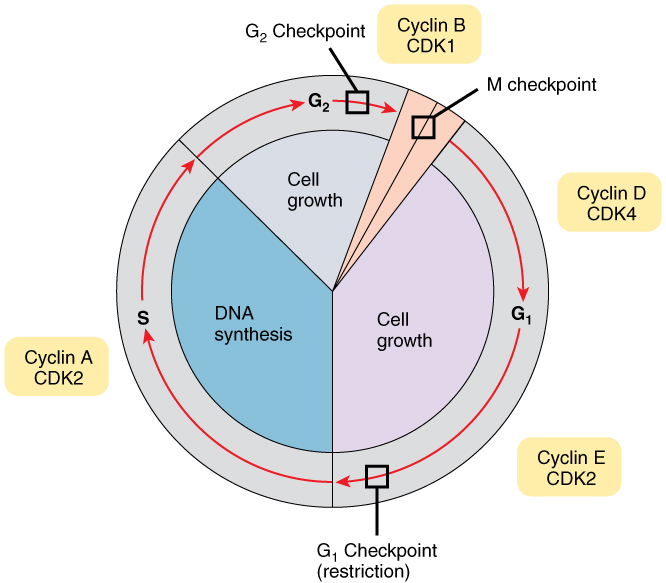
\includegraphics[width=0.5\textwidth]{Cell_Cycle}
	\caption{Representación del ciclo celular.}
	\label{fig:ciclo celular}
\end{figure}

Para nuestro modelo estableceremos que la célula pasa el \textit{punto de restricción} \footnote{El punto de restricción es el punto entre las fases $G_{1}$ y $S$, donde pasamos del crecimiento celular a la división.} (ver Figura \ref{fig:ciclo celular}) si la cantidad de Bcl-2 o de Rb cae por debajo de cierto límite, dando lugar al inicio de la muerte celular o división, respectivamente. 

La variación en las dinámicas de Rb y Bcl-2 da una explicación de la variabilidad observada en la duración de la fase $G_{1}$ de las células y, consecuentemente, en la duración de sus vidas.

\subsubsection{Los receptores de membrana regulan las dinámicas de Rb y Bcl-2}

La fluctuación en la cantidad de Rb y Bcl-2 depende de unas proteínas llamadas \textit{citoquinas} \footnote{citoquinas: son proteínas que regulan la función de las células que las producen sobre otros tipos celulares. Son los agentes responsables de la comunicación intercelular, inducen la activación de receptores específicos de membrana, funciones de proliferación y diferenciación celular, entre otros. Ver \url{https://es.wikipedia.org/wiki/Citocina}}. Estas pueden inducir tanto la fosforilación de Rb, en cuyo caso se denominan \textit{citoquinas de proliferación}. Como tener un efecto positivo o negativo en cuanto a la cantidad de Bcl-2 se refiere, en ese caso nos referiremos a ellas como \textit{citoquinas de supervivencia} o \textit{muerte}, respectivamente.

El punto importante es que la acción que las citoquinas llevan a cabo se produce gracias sus interacciones con receptores de membrana específicos. De esta manera, el efecto que percibe una célula T depende, no solo de la cantidad de citoquinas del ambiente, sino también del número de receptores de membrana de la célula. De esta manera, si, por ejemplo, tenemos una concentración muy alta de cierta citoquina, podríamos asumir que el efecto que esta va a tener en una célula T vendrá determinado por la cantidad de receptores de membrana específicos para ella que posea la célula en cuestión.

\subsubsection{Las células T naïve se dividen de manera asimétrica después de su activación.}

Postulamos que tanto los fenotipos de las células T efectoras como los de las células T con memoria se determinan durante la sinapsis inmune. Por su parte, una vez diferenciadas, las células T efectoras y con memoria, se dividen de manera simétrica y ambas pueden considerarse indistinguibles durante la respuesta inmune.


\subsection{Modelo matemático}

Basándonos en las hipótesis anteriormente formuladas proponemos a continuación una serie de ecuaciones con las que daremos forma al modelo matemático de nuestro estudio. Con este algoritmo modelaremos la decisión de las células T durante la respuesta inmune. 
Antes de expresar las ecuaciones exponemos la notación y algunas aclaraciones: 

\begin{itemize}
\item Denotaremos por \textit{$c(t)$} y \textit{$a(t)$} la cantidad de Rb y Bcl-2 activa en tiempo $t$, respectivamente.
\item Establecemos, sin pérdida de generalidad, que los límites que determinan la decisión entre división o apóptosis (ver hipótesis \ref{susubsec:hip_1}) estarán en $c(t)=0$ y $a(t)=0$, respectivamente. De acuerdo a esta hipótesis definimos: 
	\begin{itemize}
		\item \textit{Decisión}: Fase que parte desde el nacimiento de la célula hasta que una de las células inhibidoras alcanza el límite establecido.
		\item \textit{Ciclo}: Fase que se extiende desde la \textit{punto de restricción} hasta la división celular.
		\item \textit{Apóptosis}: Tiempo de vida de la célula que comprende desde la desactivación de Bcl-2 y la finalización del programa de muerte celular.
		\item \textit{División}: Estado final después de que la célula haya entrado en la fase de ciclo.
		\item \textit{Muerte}: Estado final después de haberse completado la fase de apóptosis.
	\end{itemize}
\item \textit{$R_{i}$} será el receptor de la i-ésima citoquina y \textit{$r_{i}(t)$} será la cantidad de ese receptor en tiempo $t$. 
\item $r_{T}$ es el número de señales TCR/antíeno  percibidas por la célula T correspondiente.
\item Los parámetros $\mu_{Tc}$ y $\mu_{Ta}$ denotan la tasa de cambio de las moléculas inhibidoras por cada señal del TCR. Mientras que los parámetros $\mu_{ic}$ y $\mu_{ia}$ representan la tasas de cambio del receptor $R_j$ pr cada señal $R_i$.
\item $\lambda_{Tj}$ es la tasa de cambio del receptor $R_{j}$ por cada señal del TCR. Mientras que $\lambda_{ij}$ es la tasa de cambio del receptor $R_j$ por cada señal $R_i$.
\item $k$ es el número de receptores de membrana.
\end{itemize} 

Así las cosas, ya estamos en condiciones de presentar las ecuaciones del modelo. Como ya hemos visto en la sección \ref{subsec:hip_bio}, la dinámica de los inhibidores está controlada por las señales que recibe la célula de sus receptores de membrana durante la fase de decisión. Además, este número de señales depende del número de receptores de la célula. Si ponemos todas estas hipótesis en conjunto, llegamos a unas ecuaciones como las siguientes:

\begin{equation}
	\label{sist_inhib}
	\left\{ \begin{array}{l}
	\dot{c}(t) = \mu_{Tc}r_{T}(t) + \sum_{j=1}^{k}\mu_{jc}r_{j}(t)\\
	\dot{a}(t) = \mu_{Ta}r_{T}(t) + \sum_{j=1}^{k}\mu_{ja}r_{j}(t) \\
	\end{array}
	\right.
\end{equation}

Para los receptores de membrana tenemos: 

\begin{equation}
	\label{sist_recep}
	\begin{array}{ll}
	\dot{r}_{i}(t) = \lambda_{Ti}r_{T}(t) + \sum_{j=1}^{k}\lambda_{ji}r_{j}(t) & \mbox{para $i=1,...,k$} 
	\end{array}
\end{equation}

Asumimos que los receptores de membrana involucrados en el algoritmo de decisión de las células T son independientes y tienen efectos acumulativos. De acuerdo con estas relaciones lineales obtenemos un modelo más robusto, puesto que configuraciones similares de receptores de membrana provocarán decisiones celulares similares. 

\subsubsection{Aspectos de la modelización}

\begin{itemize}
	\item Las condiciones $a(t)\geq0$, $c(t)\geq0$ y $r_i(t)\geq0$, para $i=1,...,k$ definen el domino de las ecuaciones \ref{sist_inhib} y \ref{sist_recep} durante la fase de decisión. 
	\item Cualquier receptor con valor negarivo $r_i(t)\leq0$ es \textit{reseteado} a 0 sin cambiar la fase de decisión en la que está la célula.
	\item Por su parte, las condiciones $a(t)=0$, $c(t)=0$ desencadenan el inicio de la fase de apóptosis y ciclo, respectivamente. Estas fases son excluyentes y no se pueden revertir mediante estimulación por citoquinas. Además tienen longitud constante que denotaremos por $t_{apo}$ y $t_{cycle}$.
	\item Si la célula progresa en la fase de ciclo los valores de $a(t)$ y $c(t)$ deben ser reiniciados para que las células hijas puedan comenzar la fase de decisión otra vez. 
	\item Una vez que la célula termina la fase de apóptosis es retirada de la población.
	\item Los parámetros $\lambda_{ji}$, $\mu_{ic}$, $\mu_{ia}$, $\mu_{Tc}$, $\mu_{Ta}$, $c(0)$ y $a(0)$ se consideran parámetros estructurales, es decir, se refieren a procesos biológicos que permanecen constantes durante la simulación. Mientras que los parámetros referentes a la composición de receptores de membrana para una célula concreta $r_{i0}$ dependen de la historia de encuentros con el antígeno que ha tenido su madre y diferirán entre las células hijas cuando esta se divida.
\end{itemize}


\section{Dinámica del patógeno durante la respuesta inmune}

Ahora que ya tenemos un algoritmo para la dinámica de población de las células T, modelizamos la interacción del patógeno con estas células. Debemos recordar que la dinámica de un patógeno depende en gran cantidad de las características de este. Sin embargo, en esta sección daremos unas ecuaciones muy generales para que sean aplicables a la mayor cantidad posible de situaciones:

\begin{equation}
	\label{sist_pat_T}
	\begin{array}{ll}
	\dot{y}(t) = \alpha y(t) - \beta n(t)y(t)
	\end{array}
\end{equation} 

Donde $y(t)$ y $n(t)$ denotan el número de células del patógeno y el número de células T, respectivamente. Los parámetros $\alpha$ y $\beta$ son positivos y dependen del antígeno. $\alpha$ representa la tasa de proliferación del patógeno, mientras que $\beta$ la tasa de eliminación del mismo a causa de las células T.

De acuerdo con este modelo, podemos ver que el patógeno aumenta su población hasta que el número de células T alcanza cierto valor, en ese momento $\dot{y}(t)$ se hace negativa y, en consecuencia, $y(t)$ comienza a decrecer. Asumiremos que las señales captadas por el TCR de una célula T son proporcionales al número de encuentros que tenga con el antígeno. Si llamamos al número de señales TCR de una célula $x$ en tiempo $t$, $r_{T}^{x}(t)$, tenemos:

\begin{equation}
	r_{T}^{x}(t) = \gamma\rho_{n}^{x}y(t)
\end{equation}

Donde $\gamma$ es un parámetro que depende del antígeno y denota la probabilidad de que haya una activación del TCR debido a un encuentro con el antígeno. Por otro lado,$\rho_{n}^{x}$ representa la cantidad de antígeno que está disponible para una célula T $x$. Luego:

\begin{equation}
	\sum_{x=1}^{n} \rho_{n}^{x} \leq 1
\end{equation}
	
Asumiremos también que los receptores de membrana se reparten entre las células hijas tras la división celular, de acuerdo con la siguiente ecuación:

\begin{equation}
	\left\{ \begin{array}{l}
	r_{i0}^{1}= \delta_{i}^{x} r_{i}^{x}\\
	r_{i0}^{2}= (1-\delta_{i}^{x}) r_{i}^{x} \\
	\end{array}
	\right.
\end{equation}


Donde $\delta_{i}^{x}$ representa el ratio de receptores de membrana de tipo $R_{i}$ entre las células hijas, $r_{i0}^{1}$ y $r_{i0}^{2}$ denotan los valores iniciales de receptor $R_{i}$ en las células hijas 1 y 2, respectivamente, y  $r_{i}^{x}$ denota el número de receptores $R_{i}$ en la célula T $x$ en el momento de la división celular.